%%
%% This is file `sample-sigplan.tex',
%% generated with the docstrip utility.
%%
%% The original source files were:
%%
%% samples.dtx  (with options: `all,proceedings,bibtex,sigplan')
%% 
%% IMPORTANT NOTICE:
%% 
%% For the copyright see the source file.
%% 
%% Any modified versions of this file must be renamed
%% with new filenames distinct from sample-sigplan.tex.
%% 
%% For distribution of the original source see the terms
%% for copying and modification in the file samples.dtx.
%% 
%% This generated file may be distributed as long as the
%% original source files, as listed above, are part of the
%% same distribution. (The sources need not necessarily be
%% in the same archive or directory.)
%%
%%
%% Commands for TeXCount
%TC:macro \cite [option:text,text]
%TC:macro \citep [option:text,text]
%TC:macro \citet [option:text,text]
%TC:envir table 0 1
%TC:envir table* 0 1
%TC:envir tabular [ignore] word
%TC:envir displaymath 0 word
%TC:envir math 0 word
%TC:envir comment 0 0
%%
%%
%% The first command in your LaTeX source must be the \documentclass
%% command.
%%
%% For submission and review of your manuscript please change the
%% command to \documentclass[manuscript, screen, review]{acmart}.
%%
%% When submitting camera ready or to TAPS, please change the command
%% to \documentclass[sigconf]{acmart} or whichever template is required
%% for your publication.
%% 
%%
\documentclass[sigplan,screen]{acmart}

%%
%% \BibTeX command to typeset BibTeX logo in the docs
\AtBeginDocument{%
  \providecommand\BibTeX{{%
    Bib\TeX}}}

%% Rights management information.  This information is sent to you
%% when you complete the rights form.  These commands have SAMPLE
%% values in them; it is your responsibility as an author to replace
%% the commands and values with those provided to you when you
%% complete the rights form.
\setcopyright{acmlicensed}
\copyrightyear{2018}
\acmYear{2018}
\acmDOI{XXXXXXX.XXXXXXX}

%% These commands are for a PROCEEDINGS abstract or paper.
\acmConference[Conference acronym 'XX]{Make sure to enter the correct
  conference title from your rights confirmation emai}{June 03--05,
  2018}{Woodstock, NY}
%%
%%  Uncomment \acmBooktitle if the title of the proceedings is different
%%  from ``Proceedings of ...''!
%%
%%\acmBooktitle{Woodstock '18: ACM Symposium on Neural Gaze Detection,
%%  June 03--05, 2018, Woodstock, NY}

\acmISBN{978-1-4503-XXXX-X/18/06}

%%
%% Submission ID.
%% Use this when submitting an article to a sponsored event. You'll
%% receive a unique submission ID from the organizers
%%\acmSubmissionID{123-A56-BU3}

%%
%% For managing citations, it is recommended to use bibliography
%% files in BibTeX format.
%%
%% You can then either use BibTeX with the ACM-Reference-Format style,
%% or BibLaTeX with the acmnumeric or acmauthoryear sytles, that include
%% support for advanced citation of software artefact from the
%% biblatex-software package, also separately available on CTAN.
%%
%% Look at the sample-*-biblatex.tex files for templates showcasing
%% the biblatex styles.
%%

%%
%% The majority of ACM publications use numbered citations and
%% references.  The command \citestyle{authoryear} switches to the
%% "author year" style.
%%
%% If you are preparing content for an event
%% sponsored by ACM SIGGRAPH, you must use the "author year" style of
%% citations and references.
%% Uncommenting
%% the next command will enable that style.
%%\citestyle{acmauthoryear}


\usepackage{makecell}

%%
%% end of the preamble, start of the body of the document source.
\begin{document}

%%
%% The "title" command has an optional parameter,
%% allowing the author to define a "short title" to be used in page headers.
\title{Weipipe: Weight Pipeline Parallelism for Efficient Large Language Model Training}

%%
%% The "author" command and its associated commands are used to define
%% the authors and their affiliations.
%% Of note is the shared affiliation of the first two authors, and the
%% "authornote" and "authornotemark" commands
%% used to denote shared contribution to the research.
\author{Ben Trovato}
\authornote{Both authors contributed equally to this research.}
\email{trovato@corporation.com}
\orcid{1234-5678-9012}
\author{G.K.M. Tobin}
\authornotemark[1]
\email{webmaster@marysville-ohio.com}
\affiliation{%
  \institution{Institute for Clarity in Documentation}
  \city{Dublin}
  \state{Ohio}
  \country{USA}
}

\author{Lars Th{\o}rv{\"a}ld}
\affiliation{%
  \institution{The Th{\o}rv{\"a}ld Group}
  \city{Hekla}
  \country{Iceland}}
\email{larst@affiliation.org}

%%
%% By default, the full list of authors will be used in the page
%% headers. Often, this list is too long, and will overlap
%% other information printed in the page headers. This command allows
%% the author to define a more concise list
%% of authors' names for this purpose.
\renewcommand{\shortauthors}{Trovato et al.}

%%
%% The abstract is a short summary of the work to be presented in the
%% article.
\begin{abstract}
  Abstract
\end{abstract}

%%
%% The code below is generated by the tool at http://dl.acm.org/ccs.cfm.
%% Please copy and paste the code instead of the example below.
%%

\begin{CCSXML}
<ccs2012>
 <concept>
  <concept_id>00000000.0000000.0000000</concept_id>
  <concept_desc>Do Not Use This Code, Generate the Correct Terms for Your Paper</concept_desc>
  <concept_significance>500</concept_significance>
 </concept>
 <concept>
  <concept_id>00000000.00000000.00000000</concept_id>
  <concept_desc>Do Not Use This Code, Generate the Correct Terms for Your Paper</concept_desc>
  <concept_significance>300</concept_significance>
 </concept>
 <concept>
  <concept_id>00000000.00000000.00000000</concept_id>
  <concept_desc>Do Not Use This Code, Generate the Correct Terms for Your Paper</concept_desc>
  <concept_significance>100</concept_significance>
 </concept>
 <concept>
  <concept_id>00000000.00000000.00000000</concept_id>
  <concept_desc>Do Not Use This Code, Generate the Correct Terms for Your Paper</concept_desc>
  <concept_significance>100</concept_significance>
 </concept>
</ccs2012>
\end{CCSXML}

\ccsdesc[500]{Do Not Use This Code~Generate the Correct Terms for Your Paper}
\ccsdesc[300]{Do Not Use This Code~Generate the Correct Terms for Your Paper}
\ccsdesc{Do Not Use This Code~Generate the Correct Terms for Your Paper}
\ccsdesc[100]{Do Not Use This Code~Generate the Correct Terms for Your Paper}

%%
%% Keywords. The author(s) should pick words that accurately describe
%% the work being presented. Separate the keywords with commas.
\keywords{Distributed Training, L}
%% A "teaser" image appears between the author and affiliation
%% information and the body of the document, and typically spans the
%% page.

\received{20 February 2007}
\received[revised]{12 March 2009}
\received[accepted]{5 June 2009}

%%
%% This command processes the author and affiliation and title
%% information and builds the first part of the formatted document.
\maketitle

\section{Introduction}
% 1. Transformer Arch
% 2. model is large
% 3. Challenge
% 4. Parallelism
% 5. Pipeline parallelism
% 6. Challenge Again

In recent years, advancements in transformer architectures have revolutionized the fields of natural language processing (NLP) and computer vision (CV). Scaling laws indicate a positive correlation between model performance and size. However, the growing size and complexity of these models substantially increase the requirements for computational resources. This escalation in demand necessitates more sophisticated approaches to manage and optimize the training process. 

Therefore, the deep learning community has intensely focused on distributed model training techniques designed to facilitate efficient training on vast amounts of GPUs interconnected in various topologies. To efficiently manage the computational demands of large-scale models, several parallelism strategies have been developed, such as data parallelism (DP), tensor parallelism (TP) and pipeline parallelism (PP). DP duplicates the model across all devices and performs concurrent computation on diverse inputs. TP divides matrix operations within a layer across several devices, whereas PP splits the entire model into stages processed across different devices. A notable alternative to TP is fully sharded data parallelism (FSDP), which shards parameters across devices while preserving the simplicity of DP, thereby enabling efficient large-scale training. PP offers several advantages over FSDP and TP. It reduces memory usage by distributing model stages across devices, lowering per-device memory requirements. PP also minimizes communication overhead by limiting data transfer to adjacent stages. In scenarios with limited communication bandwidth, PP has significant advantages due to its reduced need for global synchronization. These benefits make PP particularly effective for cross-server connections and scaling to thousands of GPUs.

Previous research on pipeline parallelism has predominantly focused on optimizing device idle time, known as pipeline bubbles. While reducing bubble rates is important, it is not the sole determinant of an effective pipeline parallelism strategy. Other critical factors include data communication overhead, memory utilization, load balancing, and scalability. 

% One observation is that the model size M is independent of sequence length and quadratic with the hidden dim size, while the activation size A between two decoder layers is linear with both sequence length and hidden dim size. On the wave of long context transformers, A grows much faster than M.

High communication frequency and large data transfers can negate the benefits of low bubble rates. Additionally, some strategies achieve low bubble rates at the cost of increased memory consumption, limiting model and batch sizes. Furthermore, unbalanced computation loads can lead to underutilization of resources. Therefore, a comprehensive approach that addresses these multiple aspects is essential for the development of an efficient and scalable pipeline parallelism strategy.

To address these challenges, we introduce weight pipeline parallelism, a novel strategy to optimize pipeline parallelism by representing and scheduling computations from a fresh perspective. This innovative approach aims to enhance the efficiency of PP, managing the increased volume of communication more effectively and ensuring that large models can be trained more efficiently with reduced memory consumption and improved performance. By leveraging weight parallelism, we can better utilize computational resources, ultimately advancing the capabilities of large model training. 

The contributions of this paper are as follows:

\begin{itemize}
    \item We introduce a novel pipeline parallelism scheme that improves the training efficiency of large language model with a long context.
    \item We implement a comprehensive pipeline parallelism framework using PyTorch that enabling mixed-precision training and gradient checkpointing.
    \item We proposed an interleaved schedule for weight pipeline parallelism to enhance resourse utilization and improve training efficiency significantly.
    \item Experiments on the mainstream LLama models show that WeiPipe has 20\%-50\% improvement in training efficiency compared to other pipeline parallelism strategies.
\end{itemize}

% This paper is structured as follows: Section 2 presents our handcrafted schedules based on ideal conditions, followed by Section 3, which introduces an automatic scheduling algorithm for realistic scenarios. Section 4 details a method to achieve zero bubble, preserving synchronous training semantics without synchronization during the optimizer step. Empirical evaluations against baseline methods are discussed in Section 5, and Section 6 proposes a novel scheduling mechanism to further reduce memory requirements.

\section{Background}
\subsection{Distributed Training}

\begin{figure*}[!ht]
    \centering
    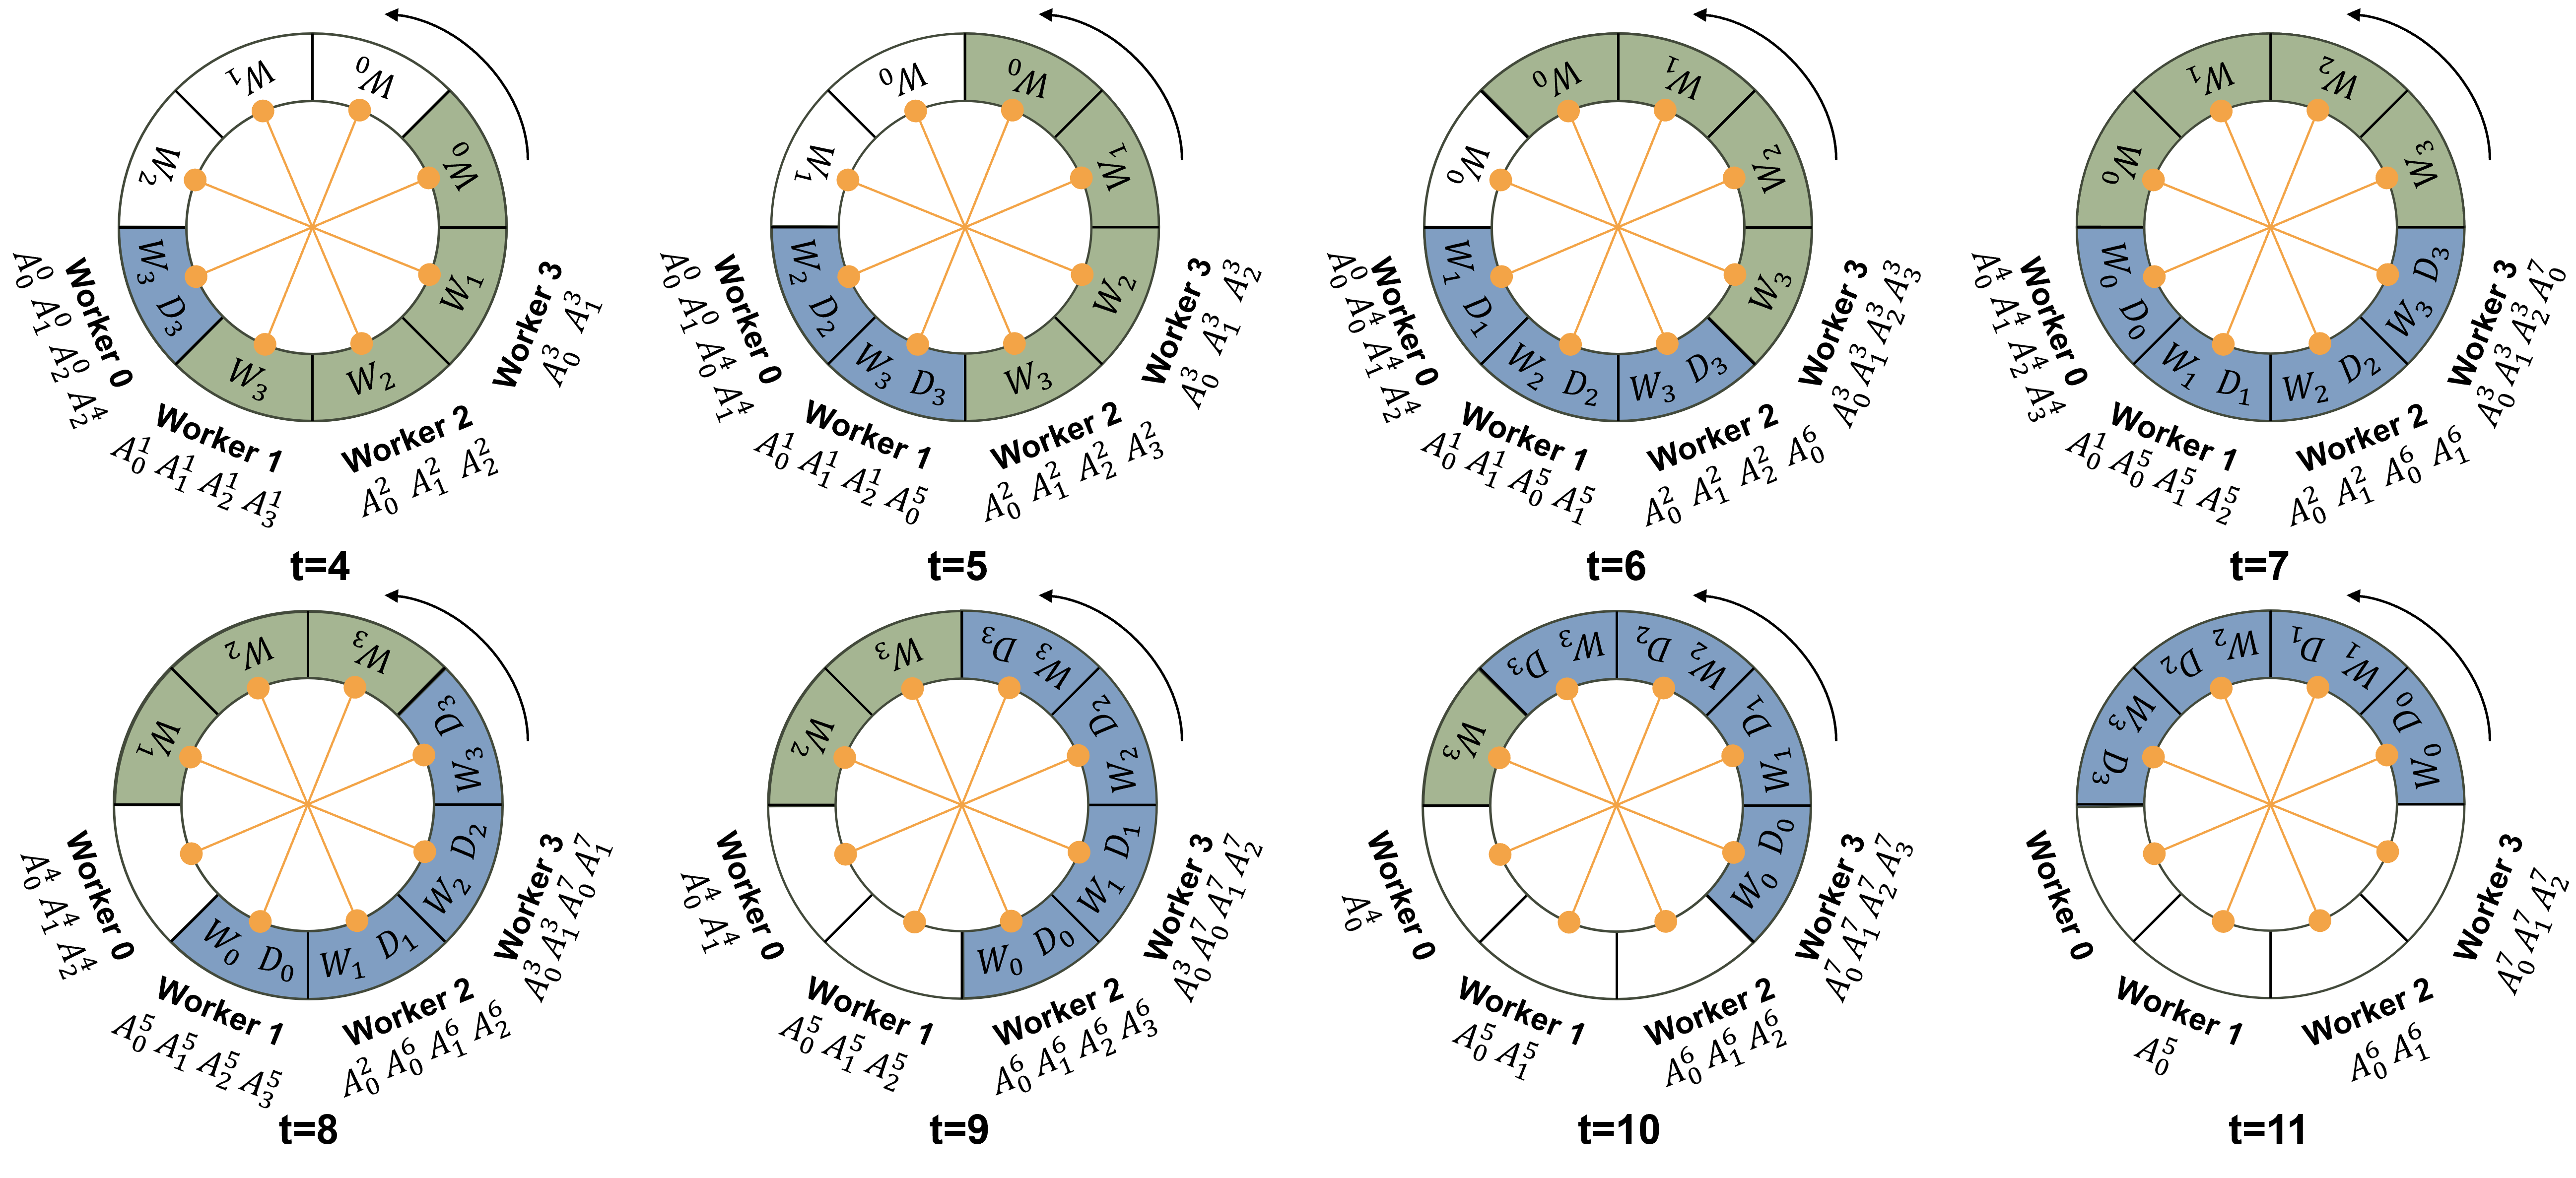
\includegraphics[scale=0.45]{figures/fig2.png}
    \caption{Pipeline parallelism}
    \label{fig:weipipe-simple}
\end{figure*}


\begin{table}[]
    \centering
    \begin{tabular}{cl}
    \toprule[1pt] 
       M  &  the number of micro-batches in a single iteration \\
       B  &  micro-batch size\\
       P  &  the number of workers \\
       L  &  the number of decoder layers in a transformer model \\
       H  &  the number of hidden dim \\
       S  &  the sequence length of the input tokens \\
       \toprule[1pt]  
    \end{tabular}
    \caption{Meaning of the symbols that are used in this paper}
    \label{tab:my_label}
\end{table}


\begin{itemize}
    \item Communication volume:  Typically, a transformer model is split into chunks when deployed into pipelined workers, with several decoder layers in each chunk. The communication volume for one activation propagation is calculated as $M_A=BLSH$. The context length $S$ of LLMs increased rapidly in recent years benefiting from the optimization of attention layers, and the micro-batch size $B$ is expected to be larger to make full use of the computation power. Therefore, the activation size $M_A$ is not a relatively small number anymore, accompanied by the increased communication cost.
    \item Memory balance: In activation pipeline parallelism, the imbalanced memory usage often leads to under-utilization of the GPU capacity. Some works fixed this problem by load balancing or adding extra pipelines. However, these works make the pipeline more complex and hard to integrate by mainstream frameworks and be used in real scenarios. Weight pipeline parallelism eliminates this problem for it has equal memory usage for every device, thus gaining a higher utilization of GPU and improving training efficiency.
\end{itemize}

\section{WeiPipe Framework} 

\subsection{Motivations}
Traditional pipeline parallelism adopts an activation-pipeline fashion. The performance advantage of pipeline parallelism compared to data parallelism is based on the data volume when conducting cross-node communication. However, this is not always true, especially in  LLM training scenarios. 

\begin{figure*}[!ht]
    \centering
    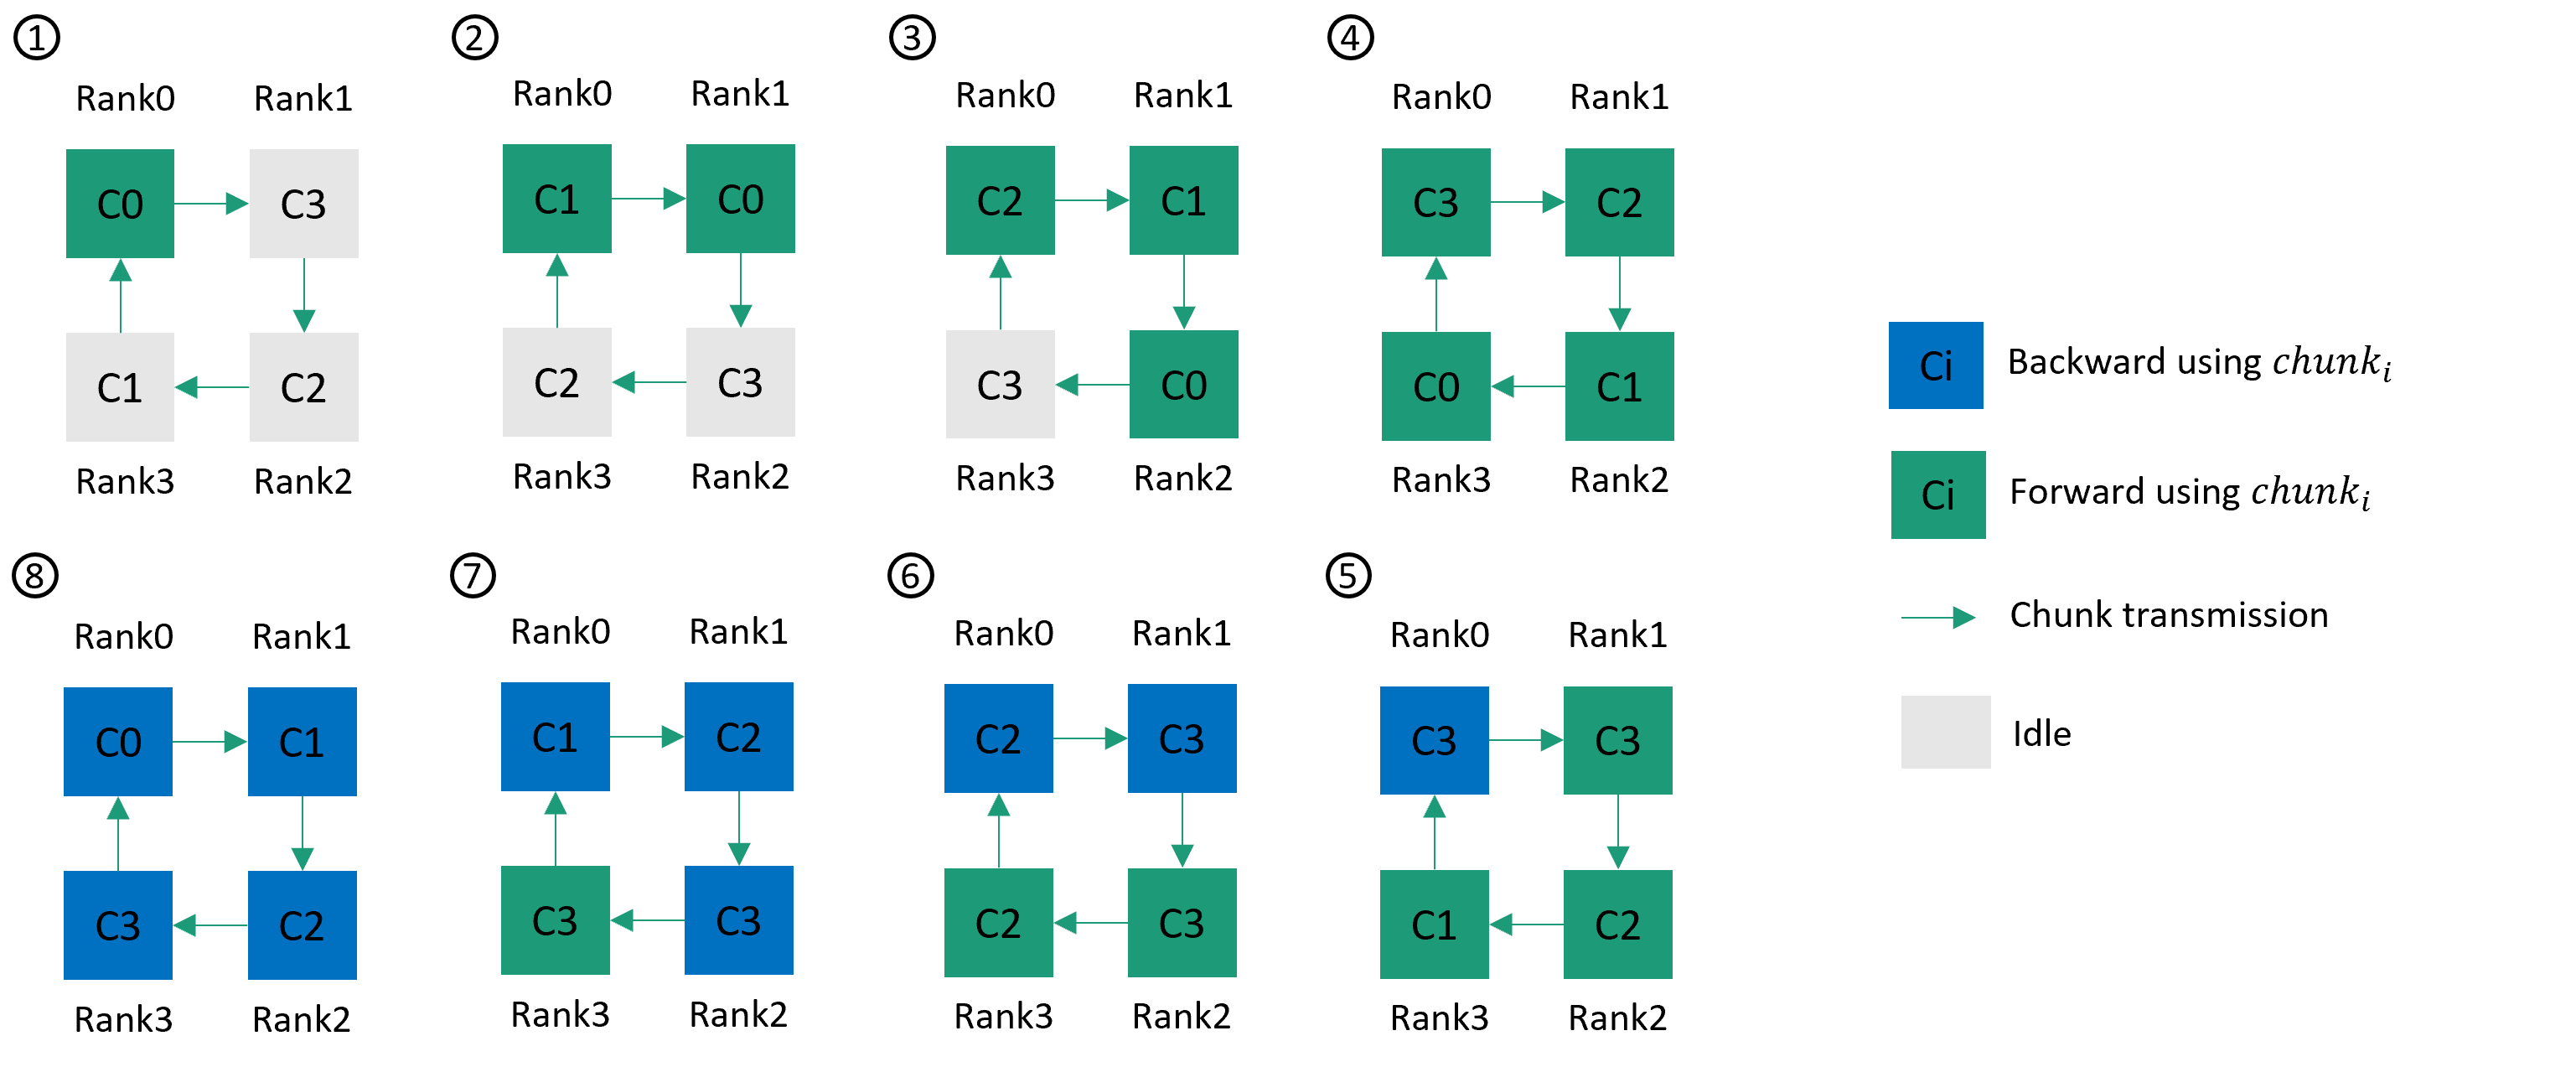
\includegraphics[scale=0.7]{figures/simple.png}
    \caption{An example of weipipe pipeline parallelism}
    \label{fig:weipipe-simple}
\end{figure*}

Considering the complexity of topology in distributed training clusters, training frameworks usually simplify this aspect. Here, we focus on the most commonly used ring topology. To minimize storage redundancy, an ideal pipeline scheme distributes the model and optimizer states evenly across all devices, akin to traditional activation pipeline parallelism. A back-propagation iteration is divided into 3 passes: a forward pass, a backward pass, and an update pass.  

In the forward pass, to ensure that the input tokens on a single device can undergo complete network computation without transferring activation values externally, we need to use inter-device communication to transfer the weights stored on the previous device to the current device, while simultaneously passing the weights stored on the current device to the next device. In a ring topology, this communication method is referred to as ring exchange. Assuming the model is divided into n chunks. For device 0, it performs the forward computation of chunk 0, 1, 2, ..., n-1 sequentially, followed by the backward computation in the order of chunk n-1, ..., 2, 1, 0, where the data of chunk is received from device n-1. For $0\le d\le n-1$,  device d waits for device d-1 to complete its computation before fetching weights from device d-1 to begin its forward computation. By exchanging chunks among all devices, Weipipe enables each device to perform computation using a complete network with 1/n storage of the weights.

In the backward pass, due to the nature of the backpropagation process itself, the weight chunks are fetched in reverse order. Throughout the pipeline computation, the smaller numbered device will complete the computation earlier relative to the larger numbered device. Therefore, when the smaller device enters the backward computation, the larger device is still performing the forward computation. The two passes exist simultaneously thus there should be another channel to transfer weights. Moreover, for any weight chunk, all devices compute a copy of the gradient of its corresponding weight on the respective batch, and these gradients need to be accumulated, thus a third channel is needed to transfer the gradients. 

In the update pass,  each device is only responsible for updating the chunk of weights it holds, and accumulated gradients are sent by the gradient channel. The update pass is performed synchronously.

\subsection{Interleaving Schedule for lower bubble ratio}  
The simple scheduling gives a feasible forward-backward-update solution. Still, the redundant transmission of weights increases the transmission cost, which further leads to a decrease in the computational utilization and affects the training efficiency. It can be observed that each device performs only one forward or backward computation when it has two weight chunks at the same time, a step that leads to a waste of resources. To fully utilize the weight chunks on the devices, the forward computation can be interspersed with the reverse computation, which results in an interleaving scheduling strategy, as shown in \ref{fig:weipipe-1f1b}.



\begin{figure*}[!ht]
    \centering
    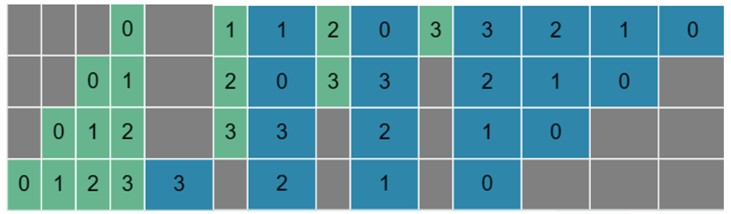
\includegraphics[scale=0.7]{figures/weipipe.jpg}
    \caption{naive weight pipeline schedule}
    \label{fig:weipipe-naive}
\end{figure*}

\begin{figure*}[!ht]
    \centering
    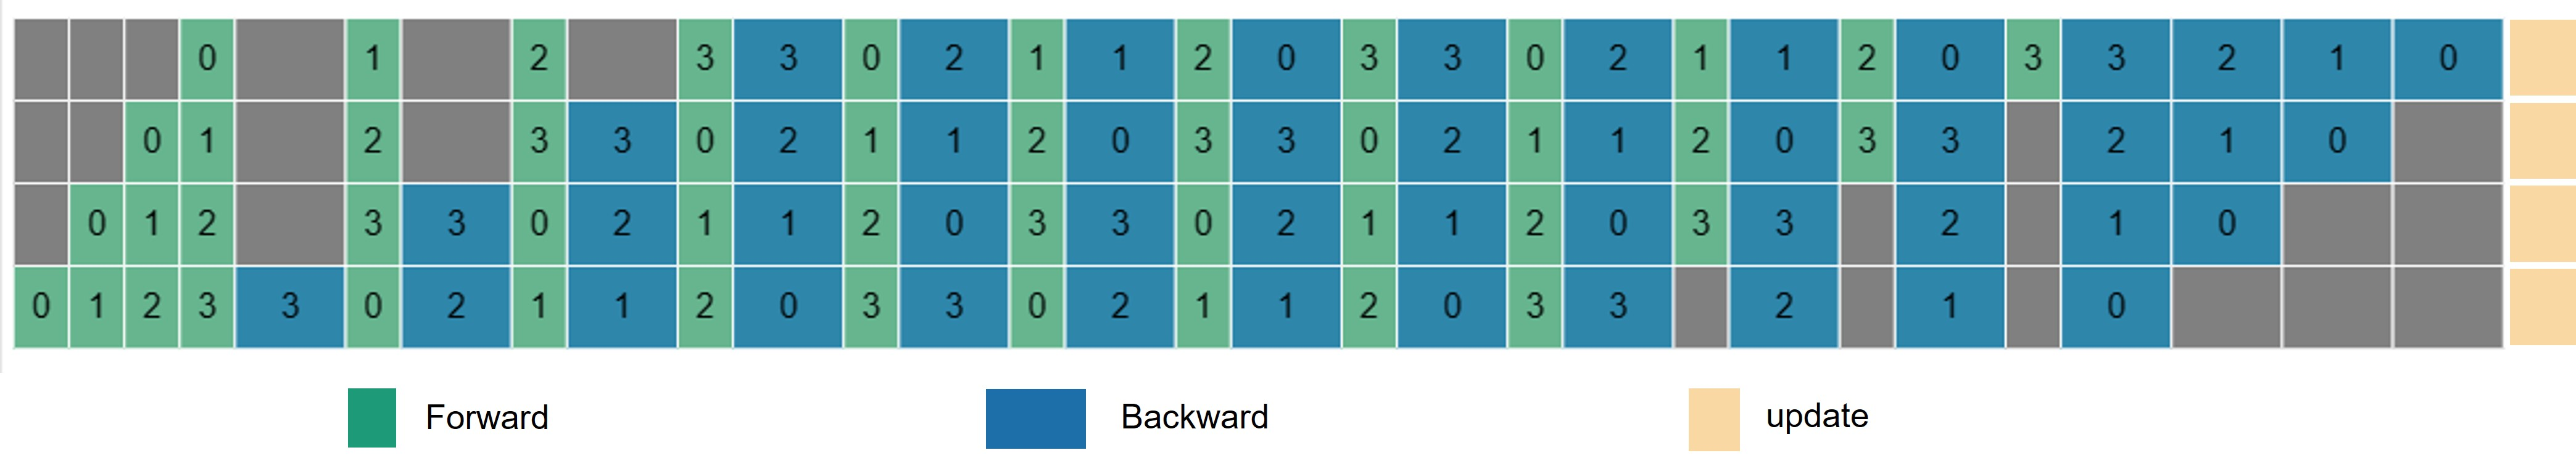
\includegraphics[scale=0.5]{figures/weipipe-1f1b.jpg}
    \caption{1F1B weight pipeline schedule}
    \label{fig:weipipe-1f1b}
\end{figure*}


% 1F1B
% latency hidden

\section{Implementation} 
Current frameworks for distributed training support pipeline parallelism and popular variants but few of them support high-level changes to the pipeline mechanism. Thus We implement WeiPipe in Pytorch from scratch, providing a specific implementation for large language model training, but this method is not limited to transformer models.

\subsection{Mixed Precision} 
Unlike other pipeline frameworks which only focus on full precision implementation, our implementable considers mixed precision optimization due to the nature of weight storage and transmission. Assuming the model size is $\phi$, the total memory occupancy is computed as 4$\phi$  :

\subsection{Overlap by prefetching}

\begin{figure*}[!ht]
    \centering
    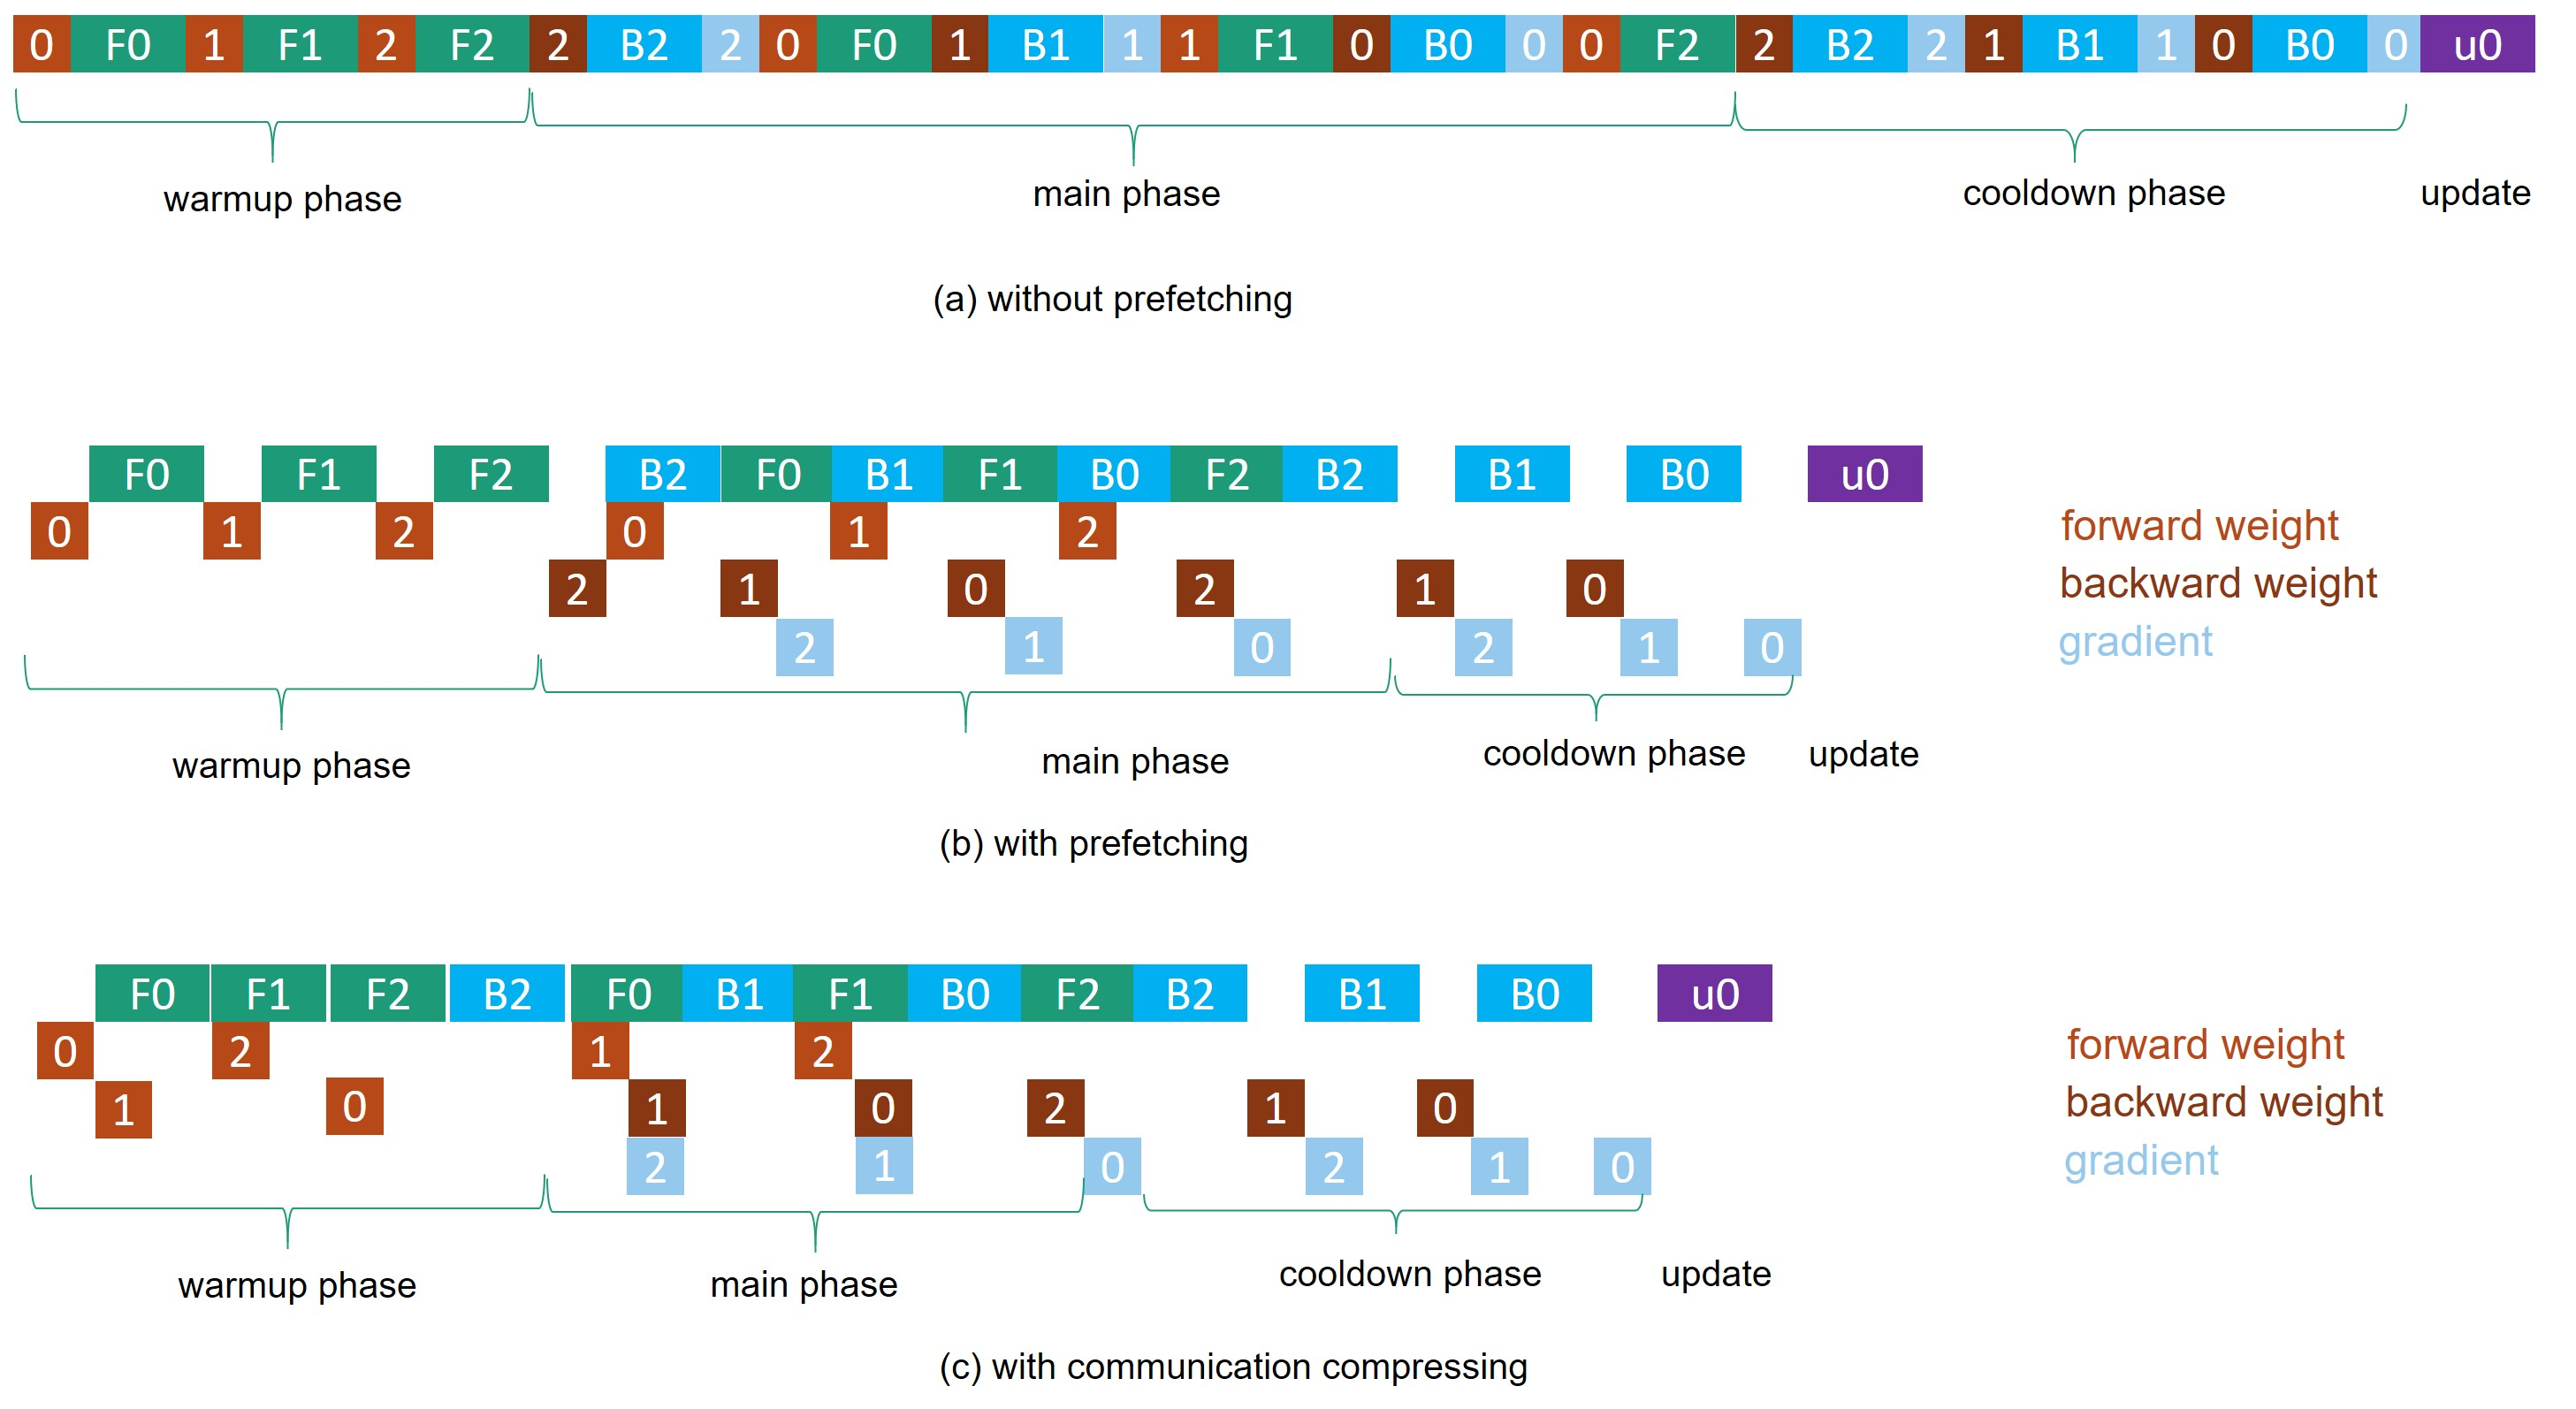
\includegraphics[scale=0.7]{figures/overlap.jpg}
    \caption{Overlap by prefetching}
    \label{fig:overlap}
\end{figure*}

The interleaving schedule requires multiple chunks of the weights to be stored on each device, and the transmission of the weights can be overlapped with the computation when performing the forward computations and the backward computations using asynchronous communication, which is realized by utilizing the batch\_isend\_irecv function provided by pytorch NCCL backend.

\section{Evaluation}
% Memory
% Speed
% Communication Volume v.s. PP
% MFU

\subsection{experimental setup}
We evaluate our implementation on models adopting the open-source LLM LLaMA architecture, as detailed in Table  \ref{tab:setting}.

compared methods:
\begin{itemize}
    \item WeiPipe: Weight pipeline with interleaved schedule 
    \item 1F1B and 1F1B-I
    \item ZB-1p and ZB-2p: zero bubble schedules are introduced by
    
\end{itemize}
The implementation of 1F1B, 1F1B-I and ZB are based on open-source Megatron-LM project. 


In the following section, we focus on addressing the following questions:
\begin{itemize}
    \item What is WeiPipe's memory consumption like in practice? 
    \item How does WeiPipe perform in diverse network scenarios?
    \item How does WeiPipe perform in weak scaling settings, where the computing resources and tasks increase simultaneously?
    \item How does Hanayo perform in strong scaling settings, where the goal is to use more computing resources to accelerate a fixed?
\end{itemize}

% peak memory consumption Figure



\begin{table*}[!ht]
    \centering
    \begin{tabular}{c|c|c|c|c|c|c|c}
    \hline
       Model  &  Layers & \makecell[c]{Attention\\Heads}  & \makecell[c]{Hidden\\Size} &\makecell[c]{Sequence\\Length}& Pipelines &  \makecell[c]{Microbatch\\Size} & \makecell[c]{ Number of \\ Microbatches }  \\
       \hline
       1.5B & 22 & 24 & 2304 & 1024 & 8 & 6 & 24/32/64 \\
       \hline
       1.5B & 22 & 24 & 2304 & 1024 & 8 & 6 & 24/32/64 \\
       \hline
       1.5B & 22 & 24 & 2304 & 1024 & 8 & 6 & 24/32/64 \\
       \hline
       1.5B & 22 & 24 & 2304 & 1024 & 8 & 6 & 24/32/64 \\
      
    \end{tabular} 
    \caption{Models and settings used in this paper}
    \label{tab:setting}
\end{table*}
    
% \subsection{comparison to data parallel}

\subsection{Adaptability Across Diverse Network Environments}
To test the adaptability of various pipeline methods in different communication environments, we prepared two test environments. 

\begin{itemize}
    \item A cloud server with 32 NVIDIA A100 GPUs that have 80GB memory. The GPUs are connected through Nvlink.
    \item A cloud server with 32 NVIDIA A100 GPUs that have 80GB memory. The GPUs are connected through PCIE. 
\end{itemize}


\subsection{Weak Scaling}
In this section, we evaluate WeiPipe’s efficiency under weak scaling settings, where we maintain the same amount of computation per device while incrementally increasing the number of devices used from 8 to 32.
The total batch size is increased from 32 to 128. In the three sets of experiments, WeiPipe outperforms 1F1B by xxx,xxx,xxx , 1F1B-I by xxx,xxx,xxx, ZB-1 by xxx,xxx,xxx, ZB-2by xxx,xxx,xxx.  

\subsection{Strong Scaling}
Strong scaling is characterized by maintaining a constant task size while increasing the number of processors. In the context of training a large language model, we attempt to use more GPUs to train the model with a fixed data batch. Here, we use a batch size of 32, which already reaches A100's 80GB memory limit. We then increase the number of GPUs from 8 to 16 and 32, examining whether the total throughput increases proportionally. The results can be found in Figure xxx. 


\section{Related Work}


\section{Conclusions}
In this work, we proposed a novel strategy for pipeline parallelism to reduce the communication overhead towards large language model training by changing the communication from activation to model weight, and we designed a 1F1B schedule for weipipe pipeline to reduce memory consumption and eliminate the overhead brought by the extra weight transportation, which greatly reduces the bubble ratio. To further enhance the max flops utilization, we designed a latency hidding strategy, which gains great performance improvement.

\section{Acknowlegment}

\begin{thebibliography}{00}
\bibitem{b1} G. Eason, B. Noble, and I. N. Sneddon, ``On certain integrals of Lipschitz-Hankel type involving products of Bessel functions,'' Phil. Trans. Roy. Soc. London, vol. A247, pp. 529--551, April 1955.
\end{thebibliography}
\end{document}
\endinput
%%
%% End of file `sample-sigplan.tex'.
